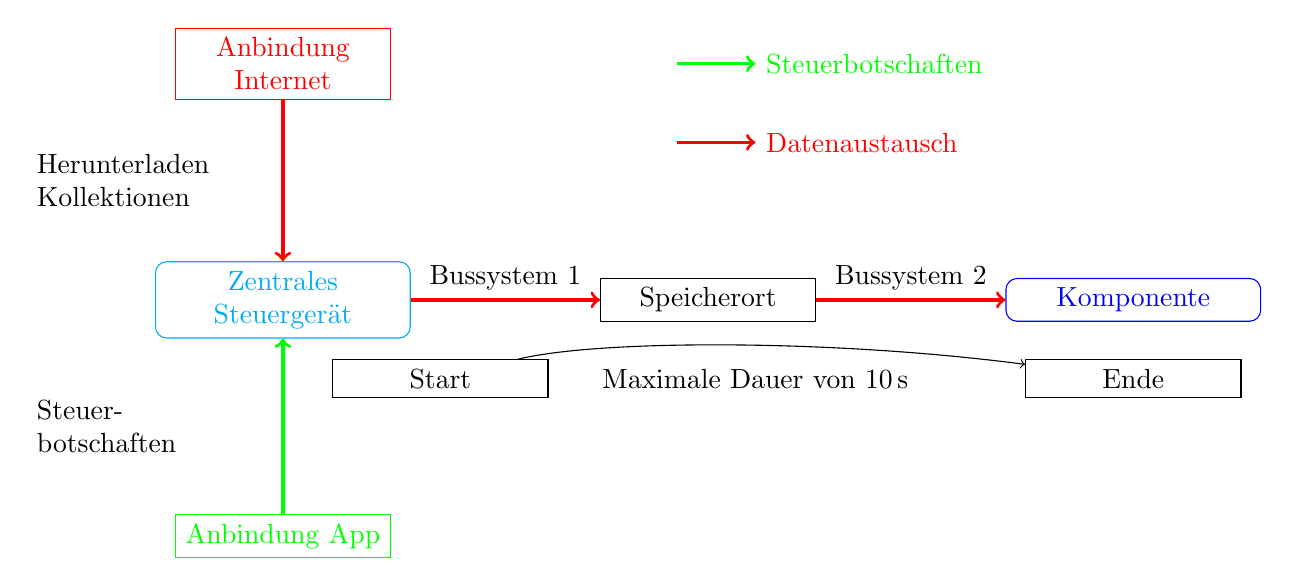
\begin{tikzpicture}[first/.style={draw, text width=3cm, align=center, rounded corners}, second/.style={draw, text width=2.5cm, align=center}]
	\node[first, cyan] (Z) at (0,0) {Zentrales Steuergerät};
	\node[second, red] (C) at (0,3) {Anbindung Internet};
	\node[second, green] (D) at (0,-3) {Anbindung App};
	\node[first, blue] (K1) at (10.8,0) {Komponente};
	\node[second] (S1) at (5.4,0) {Speicherort};
	\draw[-] (Z) -- node[left,text width=3cm] {Herunterladen Kollektionen} (C);
	\draw[-] (Z) -- node[left,text width=3cm] {Steuer-\\botschaften} (D);
	\draw[-] (Z) -- node[above] {Bussystem 1} (S1);
	\draw[-] (S1) -- node[above] {Bussystem 2} (K1.west);
	\draw[->, green, very thick] (5, 3) -- (6,3) node[right] {Steuerbotschaften};
	\draw[->, red, very thick] (5, 2) -- (6, 2) node[right] {Datenaustausch};
	\draw[->, green, very thick] (D) -- (Z);
	\draw[->, red, very thick] (C) -- (Z);
	\draw[->, red, very thick] (Z) -- (S1);
	\draw[->, red, very thick] (S1) -- (K1);
	\node[second] (S) at (2, -1) {Start};
	\node[second] (E) at (10.8, -1) {Ende};
	\draw[->] (S) .. controls (4, -0.5) and (7, -0.5) .. (E);
	\node (B) at (6,-1) {Maximale Dauer von $ 10\,\mathrm{s} $};
\end{tikzpicture}